\documentclass{standalone}
\usepackage{tikz}
\begin{document}
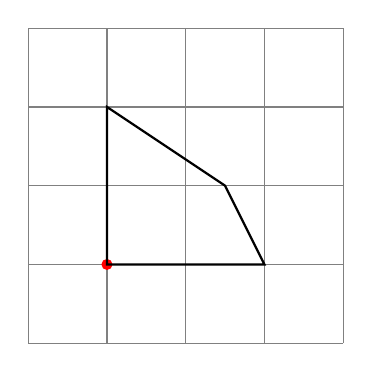
\begin{tikzpicture}[scale=1]
% 绘制背景网格
\draw[gray] (-1, -1) -- (-1, 3);
\draw[gray] (0, -1) -- (0, 3);
\draw[gray] (1, -1) -- (1, 3);
\draw[gray] (2, -1) -- (2, 3);
\draw[gray] (3, -1) -- (3, 3);
\draw[gray] (-1, -1) -- (3, -1);
\draw[gray] (-1, 0) -- (3, 0);
\draw[gray] (-1, 1) -- (3, 1);
\draw[gray] (-1, 2) -- (3, 2);
\draw[gray] (-1, 3) -- (3, 3);
\fill[red] (0,0) circle (2pt);
\draw[thick] (0,2) -- (3/2,1) -- (2,0) -- (0,0) -- cycle;
\end{tikzpicture}
\end{document}
